\chapter{Data Preparation}
\label{ch:datprep}
In questo capitolo verrà valutato come trattare al meglio i dati a disposizione per ragioni di efficienza.

\section{Selezione dei dati}
I dati saranno selezionati principalmente secondo due criteri:
\begin{itemize}
	\item Limitatezza delle risorse (tempo e strumenti di calcolo)
	\item Numero di istanze e di attributi del dataset
\end{itemize}


\section{Sampling}
\label{sec:sampling}
%BEGIN_FOLD
%Il dataset è composto da 95412 istanze, con 90569 esempi negativi e i restanti 4843 esempi positivi, quindi fortmenete sbilanciato; visto l'ingente numero e per l'obsolescenza nota della macchina di lavoro,\ si è deciso di campionare il dataset con l'algoritmo \textbf{Resample} per ottenerne uno più piccolo e più facilmente gestibile, pari al 10\% di quello originario, in più con un bias per rendere uniformi il numero di istanze positive e negative: il nuovo dataset è formato da 9541 istanze, con 4775 istanze negative e 4766 istanze positive, per via dell'uniformità.
%
%\begin{figure}[h!]
%%\begin{subfloat}
%  \begin{subfigure}{.5\textwidth}
%  \centering
%  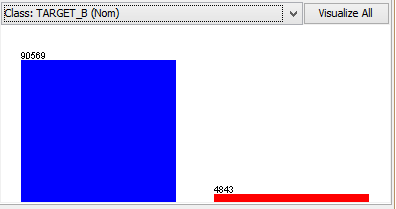
\includegraphics[width=.8\linewidth]{./images/full_unbiased}
%  \caption{Prima: integro e sbilanciato}
%  \label{fig:sfig1}
%  \end{subfigure}
%%\end{subfloat}  
%%\begin{subfloat}
%  \begin{subfigure}{.5\textwidth}
%  \centering
%  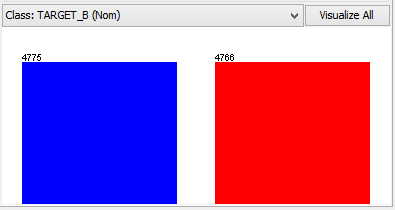
\includegraphics[width=.8\linewidth]{./images/resampled_biased}
%  \caption{Dopo: campionato e bilanciato}
%  \label{fig:sfig2}
%  \end{subfigure}
%%\end{subfloat}  
%  \caption{Versioni del dataset}	
%  \label{fig:fig}
%\end{figure}
%END_FOLD
Il dataset è composto da 95412 istanze, con 90569 esempi negativi e i restanti 4843 esempi positivi, quindi fortmenete sbilanciato. Per superare questo problema si sono svolte le seguenti fasi:
\begin{itemize}
	\item Creazione di nuove istanze per mezzo dell'algoritmo \textit{SMOTE}\cite{Chawla02smote:synthetic}, descritto nella sezione \ref{sec:construct}. Sono stati raddoppiati gli esempi positivi, passando da 4843 a 9686.
	\item Generazione di un sottoinsieme random di istanze grazie all'algoritmo \textit{SpreadSubsample}, che permette di selezionare istanze di classe di maggioranza in maniera casuale. Sono state selezionate 11623 istanze negative rispetto alle 90569 iniziali.
	\item Randomizzazione delle istanze per evitare \textit{overfitting} visto che SMOTE salva le nuove istanze della classe di minoranza in coda al file ARFF.
\end{itemize}

\begin{figure}[htbp!]
	%\begin{subfloat}
	\begin{subfigure}{.5\textwidth}
		\centering
		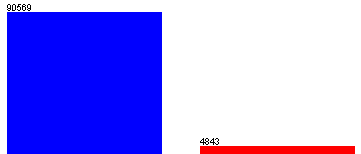
\includegraphics[width=.8\linewidth]{./images/full_unbiased2}
		\caption{Originale}
		\label{fig:unbiased}
	\end{subfigure}
	%\end{subfloat}  
	%\begin{subfloat}
	\begin{subfigure}{.5\textwidth}
		\centering
		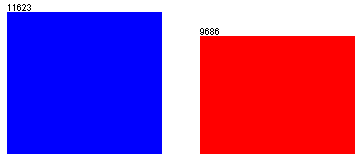
\includegraphics[width=.8\linewidth]{./images/subsampled}
		\caption{Ricampionato}
		\label{fig:sampled}
	\end{subfigure}
	%\end{subfloat}  
	\caption{Versioni del dataset}	
	\label{fig:dataset}
\end{figure}

\pagebreak

\section{Feature selection}
\label{sec:featsel}
%BEGIN_FOLD
%La feature selection ha riguardato la selezione di un sottoinsieme dei 480 attributi, un numero decisamente alto che potrebbe non apportare alcun beneficio ed anzi, potrebbe far incappare nella maledizione della dimensionalità. L'algoritmo utilizzato è l'\textbf{InfoGainAttributeEval} che, come suggerisce il nome, sfrutta la nozione di \emph{Information Gain}, cioè viene scelta la feature che apporti contenuto informativo maggiore rispetto ad un'altra. Presa in considerazione una feature X, l'\emph{Information Gain} IG(X) è definita come la differenza tra una funzione di incertezza a priori, $ \sum_i U(P(c_i)) $, e una funzione di incertezza a posteriori, data X, dove $ U $ è la funzione di incertezza e $ P(c_i) $ rappresenta la probabilità delle classi:
%
%$$ IG(X)=\sum_i U(P(c_i))-E \Big[ \sum_i(P(c_i|X)) \Big] $$
%
%Se $ U(x)=-x\log(x) $, allora $ \sum_i U(P(c_i)) $ è un misura di \textbf{entropia}. \\
%
%La quantità con cui l'entropia decresce rispecchia l'informazione aggiuntiva ottenuta dalla classe dell'attributo.
%Ad ogni attributo è assegnato un punteggio basato sull'information gain tra se stesso e l'attributo target.
%Alla fine dell'elaborazione, gli attributi rimasti sono 220:
%\begin{multicols}{5}
%	\begin{verbatim}
% 		ZIP
% 		DOB
% 		OSOURCE
% 		RFA_4
% 		RFA_3
% 		RFA_6
% 		RFA_9
% 		RFA_2
% 		RFA_8
% 		RFA_16
% 		NEXTDATE
% 		RFA_12
% 		RFA_11
% 		RFA_7
% 		RFA_5
% 		RFA_2F
% 		RFA_22
% 		MAXRDATE
% 		FISTDATE
% 		RFA_19
% 		RFA_17
% 		RFA_18
% 		RFA_14
% 		LASTGIFT
% 		MINRDATE
% 		RFA_21
% 		RFA_2A
% 		RFA_13
% 		RFA_24
% 		RFA_10
% 		LASTDATE
% 		RFA_20
% 		RFA_23
% 		MAXRAMNT
% 		AVGGIFT
% 		RAMNT_8
% 		RAMNT_14
% 		CARDGIFT
% 		PEPSTRFL
% 		MINRAMNT
% 		NGIFTALL
% 		RFA_15
% 		RAMNT_12
% 		STATE
% 		CLUSTER
% 		ODATEDW
% 		NUMPRM12
% 		RAMNT_16
% 		CARDPM12
% 		RAMNT_9
% 		CONTROLN
% 		RAMNT_13
% 		RDATE_14
% 		RAMNT_10
% 		RAMNT_19
% 		RDATE_8
% 		RAMNT_24
% 		CARDPROM
% 		NUMPROM
% 		RAMNT_11
% 		ETHC3
% 		RAMNT_18
% 		RDATE_18
% 		DOMAIN
% 		RAMNT_22
% 		RECP3
% 		RAMNT_15
% 		DMA
% 		RAMNT_7
% 		AGE905
% 		RAMNT_20
% 		POBC2
% 		EC7
% 		RDATE_3
% 		NUMCHLD
% 		RDATE_15
% 		IC15
% 		RAMNT_23
% 		HHD7
% 		EC2
% 		RAMNTALL
% 		HV2
% 		GEOCODE
% 		HVP5
% 		RDATE_19
% 		HV1
% 		HHD9
% 		HHN2
% 		ADATE_7
% 		IC4
% 		VOC2
% 		HHAS4
% 		HVP4
% 		RP1
% 		ADATE_4
% 		HHAS3
% 		RDATE_16
% 		EC1
% 		HVP3
% 		RAMNT_17
% 		HC21
% 		ETH3
% 		RDATE_22
% 		ETHC4
% 		TIMELAG
% 		HC6
% 		HVP2
% 		RDATE_20
% 		RDATE_21
% 		HC2
% 		MARR1
% 		RP3
% 		RDATE_11
% 		TPE4
% 		EC3
% 		RP4
% 		HHAS2
% 		SOLP3
% 		ETH1
% 		VOC1
% 		AGEC6
% 		RP2
% 		RDATE_24
% 		LFC10
% 		RAMNT_3
% 		OCC6
% 		RDATE_4
% 		ETHC5
% 		EC5
% 		AGE906
% 		RAMNT_21
% 		IC10
% 		MDMAUD
% 		RDATE_9
% 		LSC3
% 		RAMNT_4
% 		HHD3
% 		RDATE_6
% 		ETH4
% 		AGE902
% 		ANC2
% 		LSC4
% 		ANC3
% 		HV4
% 		EIC1
% 		OEDC4
% 		TPE12
% 		RDATE_17
% 		MAXADATE
% 		HHD4
% 		HHD1
% 		TCODE
% 		ADATE_8
% 		RDATE_13
% 		RECINHSE
% 		RDATE_7
% 		HOMEOWNR
% 		SOLIH
% 		ADATE_2
% 		AFC3
% 		INCOME
% 		CHILD18
% 		RDATE_23
% 		ADATE_18
% 		CHILD03
% 		RDATE_12
% 		MDMAUD_R
% 		WEALTH2
% 		CHILD12
% 		ADATE_3
% 		DATASRCE
% 		ADATE_12
% 		LIFESRC
% 		ADATE_6
% 		WEALTH1
% 		ADATE_11
% 		WALKER
% 		MDMAUD_F
% 		MDMAUD_A
% 		MAILCODE
% 		GENDER
% 		ADATE_10
% 		RDATE_5
% 		PETS
% 		RDATE_10
% 		NOEXCH
% 		GARDENIN
% 		ADATE_9
% 		PHOTO
% 		GEOCODE2
% 		CRAFTS
% 		ADATE_19
% 		ADATE_23
% 		CARDS
% 		BOATS
% 		ADATE_22
% 		ADATE_16
% 		ADATE_17
% 		CHILD07
% 		MAJOR
% 		ADATE_24
% 		AGEFLAG
% 		ADATE_13
% 		ADATE_14
% 		PVASTATE
% 		CATLG
% 		CDPLAY
% 		BIBLE
% 		KIDSTUFF
% 		HOMEE
% 		ADATE_21
% 		COLLECT1
% 		RECSWEEP
% 		STEREO
% 		RECPGVG
% 		FISHER
% 		PCOWNERS
% 		PLATES
% 		VETERANS
% 		TARGET_B
%LSC4
%HHD1
%HHD4
%ADATE_2
%ADATE_3
%RDATE_3
%RDATE_5
%SOLP3
%RAMNT_4
%ZIP
%RAMNT_3
%RDATE_4
%ADATE_6
%ANC2
%MDMAUD
%HHAS4
%RDATE_6
%MAXADATE
%RAMNT_20
%CONTROLN
%AFC3
%RAMNT_8
%ADATE_4
%ETHC4
%RAMNT_14
%CARDPM12
%ETH3
%RECP3
%MDMAUD_R
%DOB
%RAMNT_7
%LASTGIFT
%MAXRAMNT
%RAMNT_10
%EIC1
%OCC6
%HHD7
%RFA_2F
%RAMNT_9
%RAMNT_12
%RAMNT_13
%NOEXCH
%PEPSTRFL
%MDMAUD_A
%OSOURCE
%NGIFTALL
%RAMNT_23
%RFA_2A
%MDMAUD_F
%RAMNT_11
%AVGGIFT
%RAMNT_17
%RDATE_15
%RAMNT_18
%RAMNT_21
%RAMNT_19
%HHD9
%RAMNT_15
%RAMNT_16
%CARDPROM
%ETHC5
%RFA_2
%OEDC4
%RFA_4
%ADATE_7
%RFA_3
%CHILD03
%HHAS3
%CARDGIFT
%RDATE_14
%RAMNT_24
%MINRAMNT
%RDATE_19
%RDATE_8
%TPE4
%RFA_6
%RDATE_20
%RFA_5
%NUMPRM12
%RDATE_7
%RP1
%RFA_9
%RAMNT_22
%NUMPROM
%ADATE_23
%RFA_23
%EC7
%RAMNTALL
%RDATE_21
%RDATE_18
%RFA_8
%RFA_16
%LASTDATE
%RDATE_9
%RFA_20
%RFA_13
%RFA_12
%RFA_22
%RFA_11
%RFA_7
%VOC2
%RFA_21
%RFA_17
%RFA_19
%NUMCHLD
%MAILCODE
%CHILD18
%MAXRDATE
%CHILD12
%RFA_24
%RFA_14
%RFA_10
%RFA_18
%ETH1
%NEXTDATE
%ADATE_14
%RFA_15
%FISTDATE
%MAJOR
%ADATE_24
%ADATE_8
%DMA
%RDATE_17
%MINRDATE
%RDATE_11
%IC15
%HV2
%POBC2
%RDATE_23
%RDATE_22
%RECINHSE
%SOLIH
%LFC10
%RDATE_13
%HV1
%EC2
%MARR1
%RDATE_16
%ETHC3
%HVP3
%HVP4
%IC4
%HVP5
%HC21
%HHD3
%TPE12
%HHN2
%VOC1
%ODATEDW
%RDATE_24
%HC6
%EC3
%GEOCODE
%CARDS
%LSC3
%HC2
%AGE905
%EC1
%ETH4
%TIMELAG
%STATE
%RP4
%HVP2
%IC10
%RP3
%ADATE_19
%EC5
%AGE906
%AGEC6
%RP2
%HHAS2
%CLUSTER
%ADATE_13
%AGE902
%ADATE_10
%ANC3
%HV4
%TCODE
%INCOME
%BOATS
%ADATE_9
%RDATE_10
%ADATE_16
%DOMAIN
%CHILD07
%ADATE_18
%RDATE_12
%PHOTO
%WALKER
%HOMEOWNR
%PETS
%CRAFTS
%GARDENIN
%ADATE_12
%PVASTATE
%ADATE_11
%RECPGVG
%ADATE_17
%ADATE_22
%DATASRCE
%LIFESRC
%GENDER
%WEALTH2
%HOMEE
%WEALTH1
%KIDSTUFF
%GEOCODE2
%CATLG
%RECSWEEP
%BIBLE
%AGEFLAG
%CDPLAY
%ADATE_21
%COLLECT1
%PLATES
%STEREO
%FISHER
%PCOWNERS
%VETERANS
%TARGET_B
%	\end{verbatim}
%\end{multicols}
%END_FOLD
Come algoritmo di feature selection si è scelto il \emph{CfsSubsetEval}, che valuta il miglior subset degli attributi considerando la singola correlazione di ognuno con l'attributo di classe. Si sceglierà il subset con la più alta correlazione con l'attributo target, ma allo stesso tempo con una bassa correlazione con gli altri attributi. La ricerca nello spazio del subset degli attributi viene realizzata attraverso la strategia \textit{best first}, cercando di avvicinarsi ad un risultato ottimale in maniera \textit{greedy}, tagliando lo spazio di ricerca con la tecnica del \textit{backtracking}\cite{Hall1998}.
L'algoritmo può operare in tre modi:
\begin{itemize}
	\item Partire da un insieme di feature vuoto e incrementarlo, aggiungendo le più predittive.
	\item Partire dall'insieme contenente tutte le feature e ridurlo, eliminando quelle meno predittive.
	\item Partire da un qualsiasi punto e muoversi in entrambe le direzioni aggiungendo e rimuovendo feature.
\end{itemize}

Le feature rimanenti per \tb{} sono le seguenti:
\begin{multicols}{3}
	\begin{verbatim}
		HIT
		MALEMILI
		STATEGOV
		ETH3
		ETH6
		ETH7
		ETH8
		ETH10
		ETH14
		ETH16
		DW3
		DW8
		DW9
		HHD8
		ETHC6
		HUR1
		IC13
		TPE4
		TPE6
		TPE7
		TPE8
		PEC1
		OCC6
		OCC7
		EIC1
		EIC2
		EIC3
		EIC6
		EIC7
		EIC10
		EIC11
		EIC12
		EIC13
		OEDC5
		OEDC7
		SEC1
		SEC3
		AFC1
		AFC6
		ANC1
		ANC3
		ANC6
		ANC8
		ANC9
		ANC10
		ANC12
		ANC13
		ANC14
		ANC15
		HC3
		HC10
		HC14
		MHUC2
		AC2
		MAXADATE
		CARDPM12
		MINRAMNT
		RFA_2F
		RFA_2A
	\end{verbatim}
\end{multicols}

\section{Pulizia dei dati}
In questa fase sono stati trattate le variabili che presentano rumore e \emph{missing values}.

Il rumore si è avuto sui campi di tipo data che nel dataset originario avevano il formato "aaMM"; per risolvere i problemi sono stati rimossi gli \textit{outlier} che non rispettavano alcun formato di data conosciuto in quanto erano delle semplici cifre.

Un altro campo che conteneva degli outlier era \textit{GENDER}: tali valori sono stati rimpiazzati dalla moda.

Per quanto riguarda i missing value, sono stati rimossi gli attributi che ne contavano più del 70\%. Gli attributi rimossi sono 53.

Per gli altri attributi con il numero di missing value minore del 70\%, sono stati rimpiazzati quelli numerici dalla media dei presenti, mentre quelli categorici dalla moda.

\section{Costruzione di nuovi dati}
\label{sec:construct}
In questa fase sono state trattate due situazioni, la conversione delle date e l'incremento di istanze per mitigare lo sbilanciamento iniziale.

All'atto del caricamento del dataset in Weka, i campi di tipo data non erano trattati come tali ma come dati numerici, quindi sono stati convertiti in tipo \textit{Date}, gestito da Weka, e poi ne è stato cambiato il formato, da "aaMM" a "aaaa-MM", per una migliore gestione.

Per via della limitato numero di istanze della classe di minoranza, ne sono state generate di nuove utilizzando l'algoritmo \textit{SMOTE}.
\subsection{SMOTE}
\label{SMOTE}
SMOTE permette di ricampionare il dataset in maniera supervisionata utilizzando la \textbf{S}ynthetic \textbf{M}inority \textbf{O}versampling \textbf{TE}chnique\cite{Chawla02smote:synthetic}. Questa tecnica combina l'\emph{Information Oversampling} della classe minorante, con la \emph{Random Undersampling} della maggiorante. Di seguito l'algoritmo per effettuare il sovracampionamento della classe minorante.

\begin{algorithm}[!htb]
	\caption{\emph{SMOTE’s Informed Oversampling Procedure}}
	\begin{algorithmic}[1]
		\ForAll{Campione di minoranza}
				\State Trova i suoi $k$-viciniori di minoranza
				\State Selezionane $j$ in modo casuale
				\State Genera campioni sintetici in modo casuale unendo il campione di minoranza e i suoi $j$ viciniori ($j$ dipende dal grado di oversampling desiderato)
		\EndFor
	\end{algorithmic}
\end{algorithm}

%\pagebreak

Al termine dell'operazione le istanze di minoranza sono passate da 4843 a 9686. Successivamente verrà applicato \textit{SpreadSunsample} per ridurre il divario tra il numero delle istanze, come visto nella figura \ref{fig:sampled}.

\begin{figure}[!htb]
	\centering
	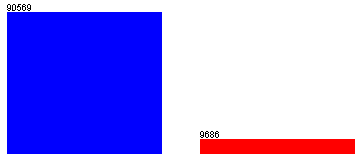
\includegraphics[width=.6\linewidth]{./images/smoted}
	\caption{Dataset dopo SMOTE, non ancora ricampionato}
\end{figure}


\section{Integrazione dei dati}
Non è stata compiuta alcuna operazione di integrazione o fusione con sorgenti dati di terze parti.

\section{Formato dei dati}
Il formato del dataset era in orgine il \textbf{Comma Separated Value} (CSV), ma per renderlo più maneggevole è stato convertito in \textbf{Attribute-Relation File Format} (ARFF).